\documentclass{article}
\usepackage{amsmath, amssymb, amsthm, graphicx, enumerate, siunitx, textgreek, multicol}
\usepackage{hyperref}
\hypersetup{
    colorlinks=true,
    linkcolor=black,
    urlcolor=blue,
}

\newcommand{\tablesection}[2] {
    \subsection{#1}  % name of the table
    #2  % description of the table
    \subsubsection{Attributes}
}

\newcommand{\attribute}[6] {
    \begin{itemize}
        \item {#1}  % attribute name
            \begin{itemize}
                \item \textbf{Description}: #2  % description of the attribute 
                \item \textbf{Data type}: #3  % data type of the attribute
                \item \textbf{Domain}: #4  % domain of the attribute
                \item \textbf{Is primary key}: #5  % is this attribute a part of the primary key?
                \item \textbf{Nullable}: #6  % is this attribute allowed to be nullable?
            \end{itemize}
    \end{itemize}
}

\setcounter{tocdepth}{2}  % limit the depth of the table of contents

\title{Magic: The Gathering Database Documentation}
\author{John Kuroda\\Akil Marshall\\Israel Trusdell}
\begin{document}
\maketitle
\newpage
\tableofcontents
\newpage

\section{Entity Relationship Diagram}
\begin{figure}[h!] % {h:here, t:top, b:bottom, p:page} add ! to override
    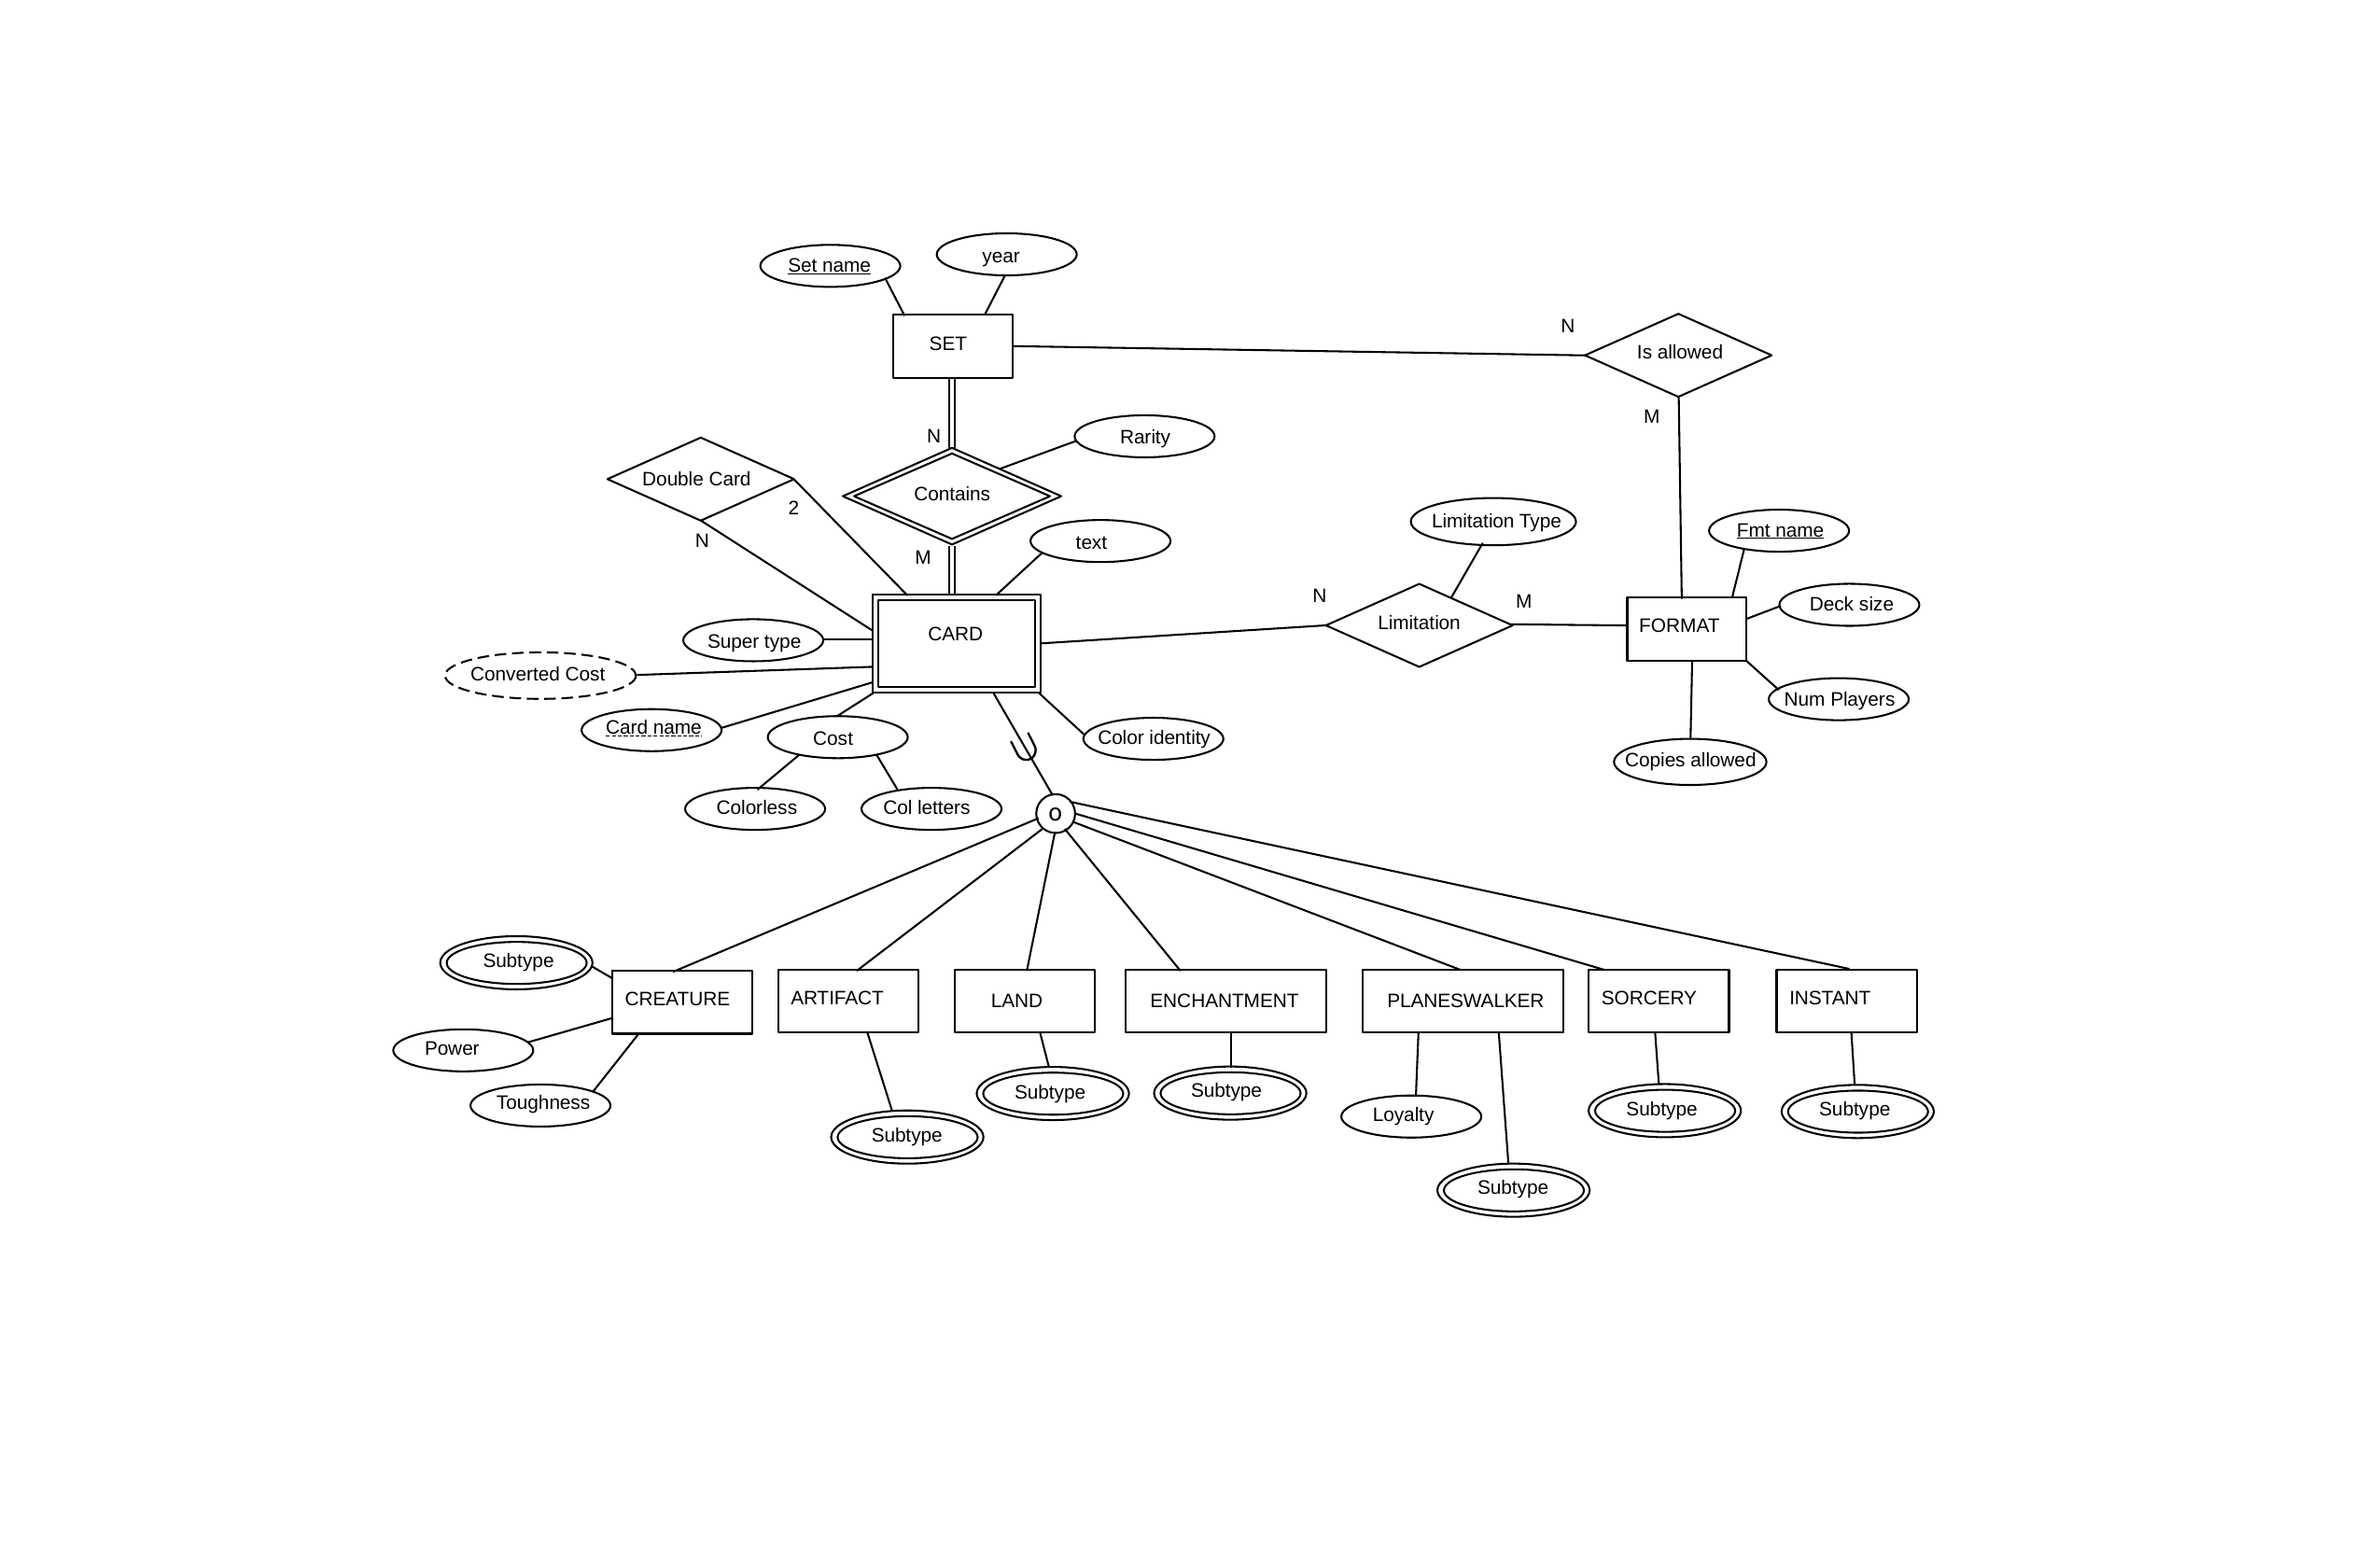
\includegraphics[width=\linewidth]{../er_diagram/er_diagram.png}
    \caption{Entity relationship diagram.}
    \label{fig:er_diagram}
\end{figure}

\section{Database Schema}
\begin{figure}[h!] % {h:here, t:top, b:bottom, p:page} add ! to override
    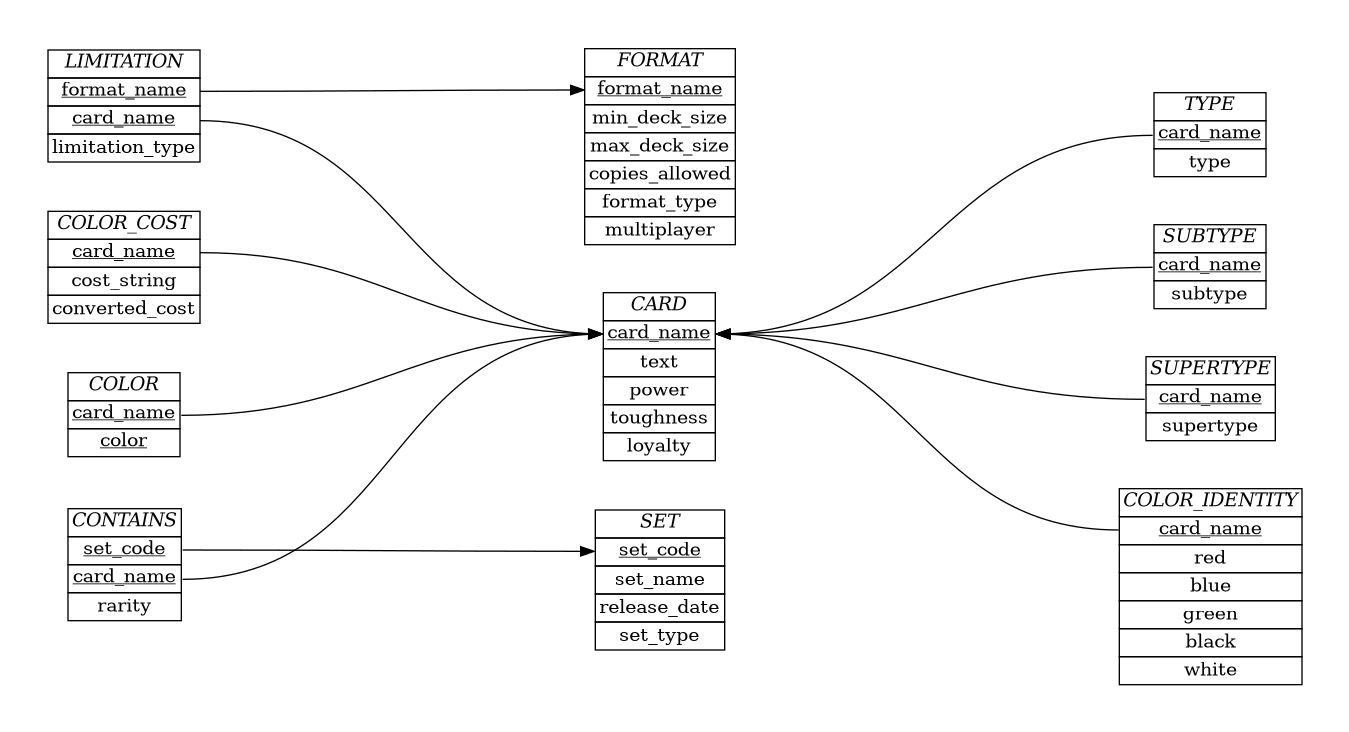
\includegraphics[width=\linewidth]{../schema/schema.png}
    \caption{Database table schema}
    \label{fig:label}
\end{figure}

\section{Efforts of Normalization}
We took our database to the third normal form.
\subsection{First Normal Form}
From the text book,
\begin{quote}
    First normal form (1NF)is now considered to be part of the formal definition of a relation in the basic (flat) relational model; historically, it was defined to disallow multivalued attributes, composite attributes, and their combinations.
    It states that the domain of an attribute must include only atomic (simple, indivisible) values and that the value of any attribute in a tuple must be a single value from the domain of that attribute.
    Hence, 1NF disallows having a set of values, a tuple o values, or a combination of both as an attribute value for a single tuple.
    In other words, 1NF disallows relations within relations or relations as attribute values within tuples. 
    The only attribute values permitted by 1NF are single atomic (or indivisible) values.
\end{quote}
Our schema is in first normal form by design.
\subsection{Second Normal Form}
From the text book,
\begin{quote}
    \textbf{Definition.} A relation schema R is in 2NF if every non-prime attribute A in R is fully functionally dependent on the primary key of R.
\end{quote}
We previously had included set\_name in the primary key of CARD.
This however violates the second normal form since the other attributes of CARD had no functional dependency on set\_name.
We then removed set\_name from CARD to bring the schema to second normal form.
\subsection{Third Normal Form}
From the text book,
\begin{quote}
    \textbf{Definition.} According to Codd’s original definition, a relation schema R is in 3NF if it satisfies 2NF and no non-prime attribute of R is transitively dependent on the primary key.
\end{quote}
Previously we had included much of the color information in the CARD table however attributes like converted\_cost were only transitively dependent on the primary key (card\_name).
To address this we created the tables COLOR, COLOR\_COST, and COLOR\_IDENTITY, moving the appropriate attributes to the correct tables.
With this each attribute depends directly on the primary key of it's table, thus our schema is in the third normal form. 

% j A CARD is the primary object this database is designed around. A CARD may be printed in one or more SETs. A SET can be uniquely identified by it's set_name or it's set_num. 
% A CARD can be in more than one set.
% CARDs are identified by their name and the SET they are printed in.
% FORMATs have a list of allowed SETs.
% CARDs can be Restricted in a FORMAT (limited to 1 copy) or Banned in a FORMAT.
% CARD is a superclass (generalization) of CREATURE, ARTIFACT, LAND, ENCHANTMENT, PLANESWALKER, SORCERY, INSTANT.
% A CARD can be in multiple subcategories, i.e., “Artifact Land”, “Artifact Creature”, or ``Enchantment Creature''.
% SETs contain CARDs.

\section{Tables}
% \subsection{FORMAT}
% FORMATs have names that identify them.
% A FORMAT is a game type with a set of rules and a list of allowed SETs.
% FORMATs also have a list of restricted cards and banned cards.  Entire sets are not necessarily illegal as a whole because cards in a set that is not allowed may show up in a set that is allowed.
% FORMATs have a predetermined deck size.
% FORMATs have a maximum number of players per game (can be $\infty$).
% \subsection{SET}
% A SET has a unique number, name, and the year it was released.
\tablesection{CARD}{
    The MTG wiki had the following to say about what a card is.
    \begin{quote}
        In Magic: The Gathering, a card is the standard component of the game. The word card usually refers to a Magic card with a Magic card front and a Magic card back, or to double-faced cards.
    \end{quote}

    The CARD table is reflective of the elements you will find on a magic card.
}
\attribute{card\_name}{The name of the card.}{String}{Any valid card name.}{Yes.}{No.}
\attribute{text}{Everything in the text area of the card.}{String}{Any valid card text.}{No.}{True}
\attribute{power}{The card's power.}{Integer}{Any non-negative integer.}{No.}{Yes.}
\attribute{toughness}{The card's toughness.}{Integer}{Any non-negative integer.}{No.}{Yes.}
\attribute{loyalty}{The card's loyalty.}{Integer}{Any non-negative integer.}{No.}{Yes.}

\tablesection{SET}{
    The MTG wiki had the following to say about what a set is.
    \begin{quote}
        A set in Magic: The Gathering is a pool of cards released together and designed for the same play environment. Cards in a set can be obtained either randomly through booster packs, or in box sets that have a fixed selection of cards. An expansion symbol and, more recently, a three-character abbreviation is printed on each card to identify the set it belongs to.
    \end{quote}

}
\attribute{set\_code}{The alphanumeric code associated with a set.}{String}{Combinations of letters and digits.}{Yes.}{No.}
\attribute{set\_name}{The name of the set.}{String}{Any valid set name.}{No.}{No}
\attribute{release\_date}{The date the set was released.}{String}{Any valid date.}{No.}{No.}
\attribute{set\_type}{The type of set it is (core, expansion, etc).}{String}{Any valid set type.}{No.}{No.}

\tablesection{FORMAT}{
    The MTG wiki had the following to say about what a format is.
    \begin{quote}
        Formats are different modes in which the Magic: The Gathering collectible card game can be played. Each format provides rules for deck construction and gameplay.
    \end{quote}
}
\attribute{format\_name}{The name of the format.}{String}{Any valid format name.}{Yes.}{No.}
\attribute{min\_deck\_size}{The minimum number of cards allowed in a deck.}{Integer}{Any non-negative integer.}{No.}{No.}
\attribute{max\_deck\_size}{The maximum number of cards allowed in a deck.}{Integer.}{Any integer, negative integers are interpreted as infinity.}{No.}{No.}
\attribute{copies\_allowed}{The maximum number of copies of a card allowed in a deck.}{Integer}{Any non-negative integer.}{No.}{No.}
\attribute{format\_type}{The type of the format (constructed, draft, etc)}{String}{Valid magic format types.}{No.}{No.}
\attribute{multiplayer}{If the format can be played by more than 2 people.}{Boolean}{Any valid boolean.}{No.}{No.}

% \tablesection{IS\_ALLOWED}{
%     This table is the implementation of the many-to-many relationship between FORMAT and SET\@. A format may allow many sets and a set may be included in many formats.
% }
% \attribute{set\_code}{A foreign key from SET.}{String}{Combinations of letters and digits.}
% \attribute{format\_name}{A foreign key from FORMAT.}{String}{Any valid format name.}

\tablesection{CONTAINS}{
    This table is the implementation of the many-to-many relationship between CARD and SET. A card may be included in may sets and A set may contain many cards.
}
\attribute{set\_code}{A foreign key from SET.}{String}{Combinations of letters and digits.}{Yes.}{No.}
\attribute{card\_name}{A foreign key from CARD.}{String}{Any valid card name.}{Yes.}{No.}
\attribute{rarity}{The rarity of the card (common, uncommon, etc).}{String}{Any valid magic card rarity.}{No.}{No.}

\tablesection{LIMITATION}{
    This table is the implementation of the many-to-many relationship between FORMAT and CARD. A format may limit many cards and a card may be limited by many formats.
}
\attribute{format\_name}{A foreign key from FORMAT.}{String}{Any valid format name.}{Yes.}{No.}
\attribute{card\_name}{A foreign key from CARD.}{String}{Any valid card name.}{Yes.}{No.}
\attribute{limitation\_type}{The way in which a card is limited (banned, restricted, etc).}{String}{Any valid limitation.}{No.}{No.}

\tablesection{COLOR}{
    MTG wiki had the following to say about color.
    \begin{quote}
        Color is a basic property of cards in Magic: The Gathering, forming the core of the game's mana system and overall strategy.
    \end{quote}
}
\attribute{card\_name}{A foreign key from CARD.}{String}{Any valid card name.}{Yes.}{No.}
\attribute{color}{The color a card is associated with, usually indicated by the physical color of the card.}{String}{Any valid magic card color.}{No.}{No.}

\tablesection{COLOR\_COST}{
    Due to the fact that converted\_cost depends on cost\_string which is not the primary key. This table solves that problem.
}
\attribute{card\_name}{A foreign key from CARD.}{String}{Any valid card name.}{Yes.}{No.}
\attribute{cost\_string}{An alphanumeric representation of a cards mana cost.}{String}{Strings over the alphabet $\sum=\{R, U, G, B, W, X, \phi\}$ where $\phi\in\mathbb{Z}_{>0}$ and each string that contains $\phi$ begins with $\phi$.}{No.}{Yes.}
\attribute{converted\_cost}{
    The sum over a cards mana cost.
    \begin{table}[h!] % {h:here, t:top, b:bottom, p:page} add ! to override
        \centering
        \caption{How to sum a cost\_string.}
        \label{tab:convertedcost}
        \begin{tabular}{cc}
            $\sum$ & value \\
            \hline
            $R$ & 1 \\
            $U$ & 1 \\
            $G$ & 1 \\
            $B$ & 1 \\
            $W$ & 1 \\
            $X$ & 0 \\
            $\phi$ & $\phi$ \\
        \end{tabular}
    \end{table}
    Each occurrence of a character in a cost\_string is summed according to the above table.
}{Integer}{Any non-negative integer.}{No.}{No.}

\tablesection{COLOR\_IDENTITY}{
    Each mana symbol that appears on a card is included within that cards color identity.
    Each card is associated with one or more colors.
}
\attribute{card\_name}{A foreign key from CARD.}{String}{Any valid card name.}{Yes.}{No.}
\attribute{red}{A flag to indicate the cards alignment with red.}{Boolean}{Any valid boolean.}{No.}{No.}
\attribute{blue}{A flag to indicate the cards alignment with blue.}{Boolean}{Any valid boolean.}{No.}{No.}
\attribute{green}{A flag to indicate the cards alignment with green.}{Boolean}{Any valid boolean.}{No.}{No.}
\attribute{white}{A flag to indicate the cards alignment with white.}{Boolean}{Any valid boolean.}{No.}{No.}
\attribute{black}{A flag to indicate the cards alignment with black.}{Boolean}{Any valid boolean.}{No.}{No.}

% \tablesection{DOUBLE\_CARD}{
%     This table allows us to describe double faced cards which are magic cards with two faces.
% }
% \attribute{side\_a}{A foreign key from CARD, specifically a card\_name.}{String}{Any valid card name.}
% \attribute{side\_b}{A foreign key from CARD, specifically a card\_name.}{String}{Any valid card name.}
% \attribute{set\_code}{A foreign key from SET.}{String}{Combinations of letters and digits.}


\tablesection{SUPERTYPE}{
    Magic cards may have one or more supertypes, this table implements that one-to-many relationship.
}
\attribute{card\_name}{A foreign key from CARD.}{String}{Any valid card name.}{Yes.}{No.}
\attribute{supertype}{The supertype of the card (legendary, snow, etc).}{String}{Any valid magic card subtype.}{No.}{No.}

\tablesection{TYPE}{
    Magic cards may have one or more types, this table implements that one-to-many relationship.
}
\attribute{card\_name}{A foreign key from CARD.}{String}{Any valid card name.}{Yes.}{No.}
\attribute{type}{The type of the card (creature, artifact, etc).}{String}{Any valid magic card type.}{No.}{No.}

\tablesection{SUBTYPE}{
    Magic cards may have zero or more subtypes, this table implements that one-to-many relationship.
}
\attribute{card\_name}{A foreign key from CARD.}{String}{Any valid card name.}{Yes.}{No.}
\attribute{subtype}{The subtype of the card (equipment, curse, etc).}{String}{Any valid magic card subtype.}{No.}{No.}

\section{Entity Constraints}
In this section we describe the constraints on entities as far as insertion, deletion, and modification are concerned.
However it must be understood that the users of this database will only be provided an interface that allows data to be read and not modified in any way.
None the less we will have a discussion on how insertions, deletions, and modifications could be done with the proposed schema.

\bigskip
It should also be noted that because of the design of Magic: the Gathering some of the following operations could never occur.
\subsection{Insertion}
\begin{description}
    \item[Card]
        To add a new card entity you must ensure that the card\_name is unique.
        However it is in the interest of the designer's of magic to ensure this is true thus you need not worry.
        In addition to the attributes in the CARD table each table that has CARD.card\_name as a foreign key must also have one or more rows populated.

        The following tables must be updated,
        \begin{multicols}{3}
            \begin{itemize}
                \item LIMITATION
                \item COLOR\_COST
                \item COLOR
                \item CONTAINS
                \item TYPE
                \item SUBTYPE
                \item SUPERTYPE
                \item COLOR\_IDENTITY
            \end{itemize}
        \end{multicols}
    \item[Format]
        To add a new format entity you must ensure that the format name is unique.
        However it is not very likely that a format will have the same name as a preexisting format.
        In addition to the attributes in the FORMAT table each table that has TABLE.format\_name as a foreign key must also have one or more rows populated.

        The following tables must be updated,
        \begin{multicols}{3}
            \begin{itemize}
                \item LIMITATION
            \end{itemize}
        \end{multicols}
        More specifically each card that is limited within the new format must be modified.
    \item[Set]
        To add a new set entity you must ensure that the set name is unique.
        However the it is in the interest of the designers of magic that each set name is unique so this isn't a problem.
        In addition to the attributes within the SET table each table that has SET.set\_name as a foreign key needs to be updated.

        The following tables must be updated,
        \begin{multicols}{3}
            \begin{itemize}
                \item CONTAINS
            \end{itemize}
        \end{multicols}
\end{description}

\subsection{Deletion}
\begin{description}
    \item[Card]
        Delete the entity within the CARD table and all tables that have the CARD.card\_name as a foreign key.

        The following tables must be checked for deletion,
        \begin{multicols}{3}
            \begin{itemize}
                \item LIMITATION
                \item COLOR\_COST
                \item COLOR
                \item CONTAINS
                \item TYPE
                \item SUBTYPE
                \item SUPERTYPE
                \item COLOR\_IDENTITY
            \end{itemize}
        \end{multicols}
    \item[Format]
        Delete the entity within the FORMAT table and all tables that have the FORMAT.format\_name as a foreign key.

        The following tables must be checked for deletion,
        \begin{multicols}{3}
            \begin{itemize}
                \item LIMITATION
            \end{itemize}
        \end{multicols}
    \item[Set]
        Delete the set entity within the SET table and all tables that have SET.set\_name as a foreign key.

        The following tables must be checked for deletion,
        \begin{multicols}{3}
            \begin{itemize}
                \item CONTAINS
            \end{itemize}
        \end{multicols}
\end{description}

% \subsection{Modification}
% To modify a record we delete it and insert a new updated version.

\section{Domain Descriptions of Certain Attributes}
In this section we either completely list the entire domain or provide examples and further description.

\subsection{SET.set\_type}
\begin{multicols}{3}
    \begin{itemize}
            \item archenemy
            \item box
            \item commander
            \item core
            \item draft\_innovation
            \item duel\_deck
            \item expansion
            \item from\_the\_vault
            \item funny
            \item masterpiece
            \item masters
            \item memorabilia
            \item planechase
            \item premium\_deck
            \item promo
            \item spellbook
            \item starter
            \item token
            \item treasure\_chest
    \end{itemize}
\end{multicols}

\subsection{CONTAINS.rarity}
\begin{multicols}{3}
    \begin{itemize}
            \item common
            \item uncommon
            \item rare
            \item mythic
    \end{itemize}
\end{multicols}

\subsection{COLOR.color}
\begin{multicols}{3}
   \begin{itemize}
           \item black
           \item blue
           \item colorless
           \item green 
           \item red
           \item white
   \end{itemize} 
\end{multicols}

\subsection{LIMITATION.limitation\_type}
\begin{multicols}{3}
    \begin{itemize}
        \item none
        \item restricted
        \item banned
    \end{itemize}
\end{multicols}
\subsection{COLOR.color}
\begin{multicols}{3}
    \begin{itemize}
        \item red
        \item green
        \item blue
        \item white
        \item black
        \item colorless
    \end{itemize}
\end{multicols}
\subsection{COLOR\_COST.cost\_string}
We provide several examples of cost\_strings.
\begin{table}[h!] % {h:here, t:top, b:bottom, p:page} add ! to override
    \centering
    \caption{Cards and their cost\_string.}
    \label{tab:coststring}
    \begin{tabular}{ll}
        Card Name & cost\_string \\
        \hline
        \href{https://scryfall.com/card/war/227/angrath-captain-of-chaos}{Angrath, Captain of Chaos} & 2B/R/R \\
        \href{https://scryfall.com/card/ori/171/conclave-naturalists}{Conclave Naturalists} & 4G \\
        \href{https://scryfall.com/card/m13/56/jace-memory-adept}{Jace, Memory Adept} & 3UU \\
        \href{https://scryfall.com/card/prm/31969/ajani-vengeant}{Ajani Vengeant} & 2RW \\
        \href{https://scryfall.com/card/bng/144/chromanticore}{Chromanticore} & WUBRG \\
    \end{tabular}
\end{table}

\subsection{SUPERTYPE.supertype}
\begin{multicols}{3}
    \begin{itemize}
        \item Basic
        \item Host
        \item Legendary
        \item Snow
        \item World
    \end{itemize}
\end{multicols}

\subsection{TYPE.type}
\begin{multicols}{3}
    \begin{itemize}
            \item artifact
            \item creature
            \item enchantment
            \item land
            \item planeswalker
            \item instant
            \item sorcery
    \end{itemize}
\end{multicols}

\subsection{SUBTYPE.subtype}
\begin{multicols}{3}
    \begin{itemize}
        \item Clue
        \item Contraption
        \item Equipment
        \item Food
        \item Fortification
        \item Gold
        \item Key
        \item Treasure
        \item Vehicle
        \item Advisor
        \item Aetherborn
        \item Ally
        \item Angel
        \item Antelope
        \item Ape
        \item Archer
        \item Archon
        \item Army
        \item Artificer
        \item Assassin
        \item Assembly-Worker
        \item Atog
        \item Aurochs
        \item Avatar
        \item Azra
        \item Badger
        \item Barbarian
        \item Basilisk
        \item Bat
        \item Bear
        \item Beast
        \item Beeble
        \item Berserker
        \item Bird
        \item Blinkmoth
        \item Boar
        \item Bringer
        \item Brushwagg
        \item Camarid
        \item Camel
        \item Caribou
        \item Carrier
        \item Cat
        \item Centaur
        \item Cephalid
        \item Chimera
        \item Citizen
        \item Cleric
        \item Cockatrice
        \item Construct
        \item Coward
        \item Crab
        \item Crocodile
        \item Cyclops
        \item Dauthi
        \item Demigod
        \item Demon
        \item Deserter
        \item Devil
        \item Dinosaur
        \item Djinn
        \item Dragon
        \item Drake
        \item Dreadnought
        \item Drone
        \item Druid
        \item Dryad
        \item Dwarf
        \item Efreet
        \item Egg
        \item Elder
        \item Eldrazi
        \item Elemental
        \item Elephant
        \item Elf
        \item Elk
        \item Eye
        \item Faerie
        \item Ferret
        \item Fish
        \item Flagbearer
        \item Fox
        \item Frog
        \item Fungus
        \item Gargoyle
        \item Germ
        \item Giant
        \item Gnome
        \item Goat
        \item Goblin
        \item God
        \item Golem
        \item Gorgon
        \item Graveborn
        \item Gremlin
        \item Griffin
        \item Hag
        \item Harpy
        \item Hellion
        \item Hippo
        \item Hippogriff
        \item Homarid
        \item Homunculus
        \item Horror
        \item Horse
        \item Hound
        \item Human
        \item Hydra
        \item Hyena
        \item Illusion
        \item Imp
        \item Incarnation
        \item Insect
        \item Jackal
        \item Jellyfish
        \item Juggernaut
        \item Kavu
        \item Kirin
        \item Kithkin
        \item Knight
        \item Kobold
        \item Kor
        \item Kraken
        \item Lamia
        \item Lammasu
        \item Leech
        \item Leviathan
        \item Lhurgoyf
        \item Licid
        \item Lizard
        \item Manticore
        \item Masticore
        \item Mercenary
        \item Merfolk
        \item Metathran
        \item Minion
        \item Minotaur
        \item Mole
        \item Monger
        \item Mongoose
        \item Monk
        \item Monkey
        \item Moonfolk
        \item Mouse
        \item Mutant
        \item Myr
        \item Mystic
        \item Naga
        \item Nautilus
        \item Nephilim
        \item Nightmare
        \item Nightstalker
        \item Ninja
        \item Noble
        \item Noggle
        \item Nomad
        \item Nymph
        \item Octopus
        \item Ogre
        \item Ooze
        \item Orb
        \item Orc
        \item Orgg
        \item Ouphe
        \item Ox
        \item Oyster
        \item Pangolin
        \item Peasant
        \item Pegasus
        \item Pentavite
        \item Pest
        \item Phelddagrif
        \item Phoenix
        \item Pilot
        \item Pincher
        \item Pirate
        \item Plant
        \item Praetor
        \item Prism
        \item Processor
        \item Rabbit
        \item Rat
        \item Rebel
        \item Reflection
        \item Rhino
        \item Rigger
        \item Rogue
        \item Sable
        \item Salamander
        \item Samurai
        \item Sand
        \item Saproling
        \item Satyr
        \item Scarecrow
        \item Scion
        \item Scorpion
        \item Scout
        \item Sculpture
        \item Serf
        \item Serpent
        \item Servo
        \item Shade
        \item Shaman
        \item Shapeshifter
        \item Sheep
        \item Siren
        \item Skeleton
        \item Slith
        \item Sliver
        \item Slug
        \item Snake
        \item Soldier
        \item Soltari
        \item Spawn
        \item Specter
        \item Spellshaper
        \item Sphinx
        \item Spider
        \item Spike
        \item Spirit
        \item Splinter
        \item Sponge
        \item Squid
        \item Squirrel
        \item Starfish
        \item Surrakar
        \item Survivor
        \item Tentacle
        \item Tetravite
        \item Thalakos
        \item Thopter
        \item Thrull
        \item Treefolk
        \item Trilobite
        \item Triskelavite
        \item Troll
        \item Turtle
        \item Unicorn
        \item Vampire
        \item Vedalken
        \item Viashino
        \item Volver
        \item Wall
        \item Warlock
        \item Warrior
        \item Weird
        \item Werewolf
        \item Whale
        \item Wizard
        \item Wolf
        \item Wolverine
        \item Wombat
        \item Worm
        \item Wraith
        \item Wurm
        \item Yeti
        \item Zombie
        \item Zubera
        \item Aura
        \item Carouche
        \item Curse
        \item Saga
        \item Shrine
        \item Plains
        \item Island
        \item Swamp
        \item Mountain
        \item Forest
        \item Desert
        \item Gate
        \item Lair
        \item Locus
        \item Urza's
        \item Mine
        \item Power-Plant
        \item Tower
        \item Ajani
        \item Aminatou
        \item Angrath
        \item Arlinn
        \item Ashiok
        \item Bolas
        \item Chandra
        \item Dack
        \item Daretti
        \item Davriel
        \item Domri
        \item Dovin
        \item Elspeth
        \item Estrid
        \item Freyalise
        \item Garruk
        \item Gideon
        \item Huatli
        \item Jace
        \item Jaya
        \item Karn
        \item Kasmina
        \item Kaya
        \item Kiora
        \item Koth
        \item Liliana
        \item Nahiri
        \item Narset
        \item Nissa
        \item Nixilis
        \item Oko
        \item Ral
        \item Rowan
        \item Saheeli
        \item Samut
        \item Sarkhan
        \item Serra
        \item Sorin
        \item Tamiyo
        \item Teferi
        \item Teyo
        \item Tezzeret
        \item Tibalt
        \item Ugin
        \item Venser
        \item Vivien
        \item Vraska
        \item Will
        \item Windgrace
        \item Wrenn
        \item Xenagos
        \item Yanggu
        \item Yanling
        \item Adventure
        \item Arcane
        \item Trap
        \item Adventure
        \item Arcane
    \end{itemize}
\end{multicols}
\end{document}
